\documentclass[12pt,fleqn]{article}

\usepackage{fullpage}
\usepackage[round]{natbib}
\usepackage{multirow}
\usepackage{booktabs}
\usepackage{tabularx}
\usepackage{graphicx}
\usepackage{float}
\usepackage{hyperref}
\hypersetup{
    colorlinks,
    citecolor=black,
    filecolor=black,
    linkcolor=black,
    urlcolor=blue
}

\newcounter{acnum}
\newcommand{\actheacnum}{AC\theacnum}
\newcommand{\acref}[1]{AC\ref{#1}}

\newcounter{ucnum}
\newcommand{\uctheucnum}{UC\theucnum}
\newcommand{\uref}[1]{UC\ref{#1}}

\newcounter{mnum}
\newcommand{\mthemnum}{M\themnum}
\newcommand{\mref}[1]{M\ref{#1}}



\pagenumbering{arabic}
\newcounter{stepnum}


\title{Module Guide}

\author{
Alex Trudeau\\
	\texttt{400030148}
\and
Kathryn Kodama\\
  	\texttt{400013582}
\and
Tommy Tran\\
	\texttt{001150067}
}


\date{\today\\ Version 1.2}

\begin{document}

\maketitle

\pagebreak

\tableofcontents
\listoftables
\listoffigures
\begin{table}[ht]
\caption{\bf Revision History}
\begin{tabularx}{\textwidth}{p{3cm}p{2cm}X}
\toprule {\bf Date} & {\bf Version} & {\bf Notes}\\
\midrule
November 6, 2017 & 1.0 & Created\\
November 8, 2017 & 1.1 & Updated content\\
November 10, 2017 & 1.2 & Updated and finalized content \\
\bottomrule
\end{tabularx}
\end{table}


\pagebreak


\section{Introduction}
Reddit Clone is a project that mimics the basic functionality of the website Reddit, a community based social news aggregator. This document(referred to as the Module Guide) aims to specify the module structure of the system for designers and maintainers. In order to support the principle of information hiding, the system is decomposed into easily maintainable, reusable modules with low coupling and high cohesion.\\
\\
The following is an outline of the document structure:
\begin{itemize}
    \item Section \ref{sec:changes} contains possible changes to the system
    \item Section \ref{sec:hierarchy} provides an overview of module design within the system
    \item Section \ref{sec:connection} explains how the requirements and module design are related
    \item Section \ref{sec:md} provides details on each module, specifically it's  secret(s) and service(s)
    \item Section \ref{sec:tracematrix} contains the traceability matrices between modules/requirements and modules/anticipated changes
    \item Section \ref{sec:usehierarchy} provides the use hierarchy between each module
    
\end{itemize}

MIS documentation was generated for each module and markdown document.  The MIS was generated using CompoDoc, a document generator for AngularJS projects.  MIS documentation can be found in the \href{https://gitlab.cas.mcmaster.ca/trudeaua/reddit-clone/tree/master/Documentation/MIS}{Gitlab repo}.

\section{Anticipated and Unlikely Changes} \label{sec:changes}
\subsection{Anticipated Changes} \label{subsec:anticipated}
\begin{description}
\item[\refstepcounter{acnum} \actheacnum:] Navigation methods
\item[\refstepcounter{acnum} \actheacnum:] Data modelling
\item[\refstepcounter{acnum} \actheacnum:] Content interaction
\item[\refstepcounter{acnum} \actheacnum:] Data management
\end{description}

\subsection{Unlikely Changes} \label{SecUchange}
\begin{description}
\item[\refstepcounter{ucnum} \uctheucnum:] Input/Output devices of the system
\item[\refstepcounter{ucnum} \uctheucnum:] Real time database/hosting using Firebase
\item[\refstepcounter{ucnum} \uctheucnum:] Assumption of a working internet connection
\item[\refstepcounter{ucnum} \uctheucnum:] User interface
\item[\refstepcounter{ucnum} \uctheucnum:] Authentication methods
\item[\refstepcounter{ucnum} \uctheucnum:] Ability to edit posts/subreddits/user profiles
\end{description}

\section{Module Hierarchy} \label{sec:hierarchy}

This section provides an overview of module design within the system, including naming and classifications . Modules are summarized
in a hierarchy decomposed by secrets in Table \ref{TblMH}. The modules listed
below, which are leaves in the hierarchy tree are the modules that will
actually be implemented.

\begin{table}[!htbp]
	\begin{tabular}{ll}
		\toprule
		Module Name & Module Number \\
		\midrule
		Hardware Hiding Module & M1\\
		\midrule
		Authentication Module & M2\\
		\midrule
		Subreddit Module & M3\\
		\midrule
		Searching Module & M4\\
		\midrule
		Post Module & M5\\
		\midrule
		Comment Module & M6\\
		\midrule
		Storage Module & M7\\
		\midrule
		Sorting Module & M8\\
		\midrule
		Database Module & M9\\
		\midrule
		Database Module & M10\\
		\bottomrule
	\end{tabular}
	\caption{Module Number Format}
	% Colour for the rulings in tables:
	\makeatletter
	\def\rulecolor#1#{\CT@arc{#1}}
	\def\CT@arc#1#2{%
		\ifdim\baselineskip=\z@\noalign\fi
		{\gdef\CT@arc@{\color#1{#2}}}}
	\let\CT@arc@\relax
	\makeatother
	\label{Table 1}
\end{table}

\vspace{5mm}

\begin{table}[h!]
\centering
\begin{tabular}{p{0.3\textwidth} p{0.6\textwidth}}
\toprule
\textbf{Level 1} & \textbf{Level 2}\\
\midrule

{Hardware-Hiding Module} & ~ \\
\midrule

\multirow{5}{0.3\textwidth}{Behaviour-Hiding Module} 
& Authentication Module (M2)\\
& Searching Module (M4)\\
& Storage Module (M7)\\
& Sorting Module (M8)\\ 
& Database Module (M9)\\
\midrule

\multirow{3}{0.3\textwidth}{Software Decision Module}
& Subreddit Module (M3)\\
& Post Module (M5)\\
& Comment Module (M6)\\
& Homepage Module (M10)\\
\bottomrule

\end{tabular}
\caption{Module Hierarchy}
\label{TblMH}
\end{table}
\newpage

\section{Connection Between Requirements and Design} \label{sec:connection}

The system is designed to satisfy the requirements stated in the Software Requirements Specification (SRS) as well as allow for further features to be added. The user interface mimics the appearance of the original Reddit's mobile site and is designed to be intuitive and easy to use for most users. A graphical representation of the connection between the requirements listed in the SRS and the modules specified within this document can be viewed in Table \ref{table:reqmodules}.

\section{Module Decomposition} \label{sec:md}



% Modules are decomposed according to the principle of ``information hiding''
% proposed by \citet{ParnasEtAl1984}. The \emph{Secrets} field in a module
% decomposition is a brief statement of the design decision hidden by the
% module. The \emph{Services} field specifies \emph{what} the module will do
% without documenting \emph{how} to do it. For each module, a suggestion for the
% implementing software is given under the \emph{Implemented By} title. If the
% entry is \emph{OS}, this means that the module is provided by the operating
% system or by standard programming language libraries.  Also indicate if the
% module will be implemented specifically for the software.

% Only the leaf modules in the
% hierarchy have to be implemented. If a dash (\emph{--}) is shown, this means
% that the module is not a leaf and will not have to be implemented. Whether or
% not this module is implemented depends on the programming language
% selected.

\subsection{Hardware Hiding Modules}

\begin{description}
\item[Secrets:] The implementation of the virtual machine within device being used
\item[Services:]Interface between user and the system
\item[Implemented By:] Internet browser
\end{description}

\subsection{Behaviour-Hiding Module}

\subsubsection{Authentication Module}
\begin{description}
\item[Secrets:] Authentication
\item[Services:] This module contains all the logic that handles authenticating user and setting user environment variables. 
\item[Implemented By:] --
\end{description}

\subsubsection{Searching Module}
\begin{description}
\item[Secrets:] Searching algorithm
\item[Services:] Handles searching for subreddits within the application 
\item[Implemented By:] --
\end{description}

\subsubsection{Storage Module}
\begin{description}
\item[Secrets:] User settings
\item[Services:] Contains user settings on local machine
\item[Implemented By:] --
\end{description}

\subsubsection{Sorting Module}
\begin{description}
\item[Secrets:] Sorting algorithms
\item[Services:] Sorts posts based off of different attributes
\item[Implemented By:] --
\end{description}

\subsubsection{Database Module}
\begin{description}
\item[Secrets:] Database communication
\item[Services:] Handles users adding, deleting or updating content
\item[Implemented By:] --
\end{description}

\subsubsection{Homepage Module}
\begin{description}
\item[Secrets:] Main hub to all features
\item[Services:] Central navigation and access to all features or content
\item[Implemented By:] --
\end{description}

\subsubsection{User Authentication Module}
\begin{description}
\item[Secrets: ] User authentication communication
\item[Services: ] Handling new users, creation of users, password and username authentication, password reset
\item[Implemented By: ] --
\end{description}


\subsection{Software Decision Module}

\subsubsection{Subreddit Module}
\begin{description}
\item[Secrets:] The design decision of how to navigate to and from subreddits as well as how content is created or loaded and displayed
\item[Services:] Displaying a page specific to a certain topic
\item[Implemented By:] --
\end{description}

\subsubsection{Post Module}
\begin{description}
\item[Secrets:] The design decision of how to navigate to and from posts as well as loading post content
\item[Services:] Displaying post content
\item[Implemented By:] --
\end{description}

\subsubsection{Comment Module}
\begin{description}
\item[Secrets:] The design decision of how to navigate to and from the comments page as well as how to load and display comments
\item[Services:] Displaying comments specific to posts selected
\item[Implemented By:] --
\end{description}

\section{Traceability Matrix} \label{sec:tracematrix}

\begin{table}[H]
\centering
\caption{Trace Between Requirements and Modules}
\label{table:reqmodules}
\begin{tabular}{p{0.2\textwidth} p{0.5\textwidth}}
\toprule
        Requirement & Modules \\
        \midrule
        \multicolumn{1}{c}{Functional Requirements} \\
        \midrule
        FR1 & M2, M9, M10 \\
        FR2 & M2, M3 \\
        FR3 & M3, M5, M6, M9, M10 \\
        FR4 & M2, M5, M6, M9 \\
        FR5 & M2, M6, M9 \\
        FR6 & M2, M5, M6, M9, M10 \\
        FR7 & M3, M7, M8, M9, M10 \\
        FR8 & M9, M10 \\
        \midrule
        \multicolumn{1}{c}{Non-functional Requirements} \\
        \midrule
        NF1 & M3, M5, M6, M8, M10 \\
        NF2 & M1 \\
        NF3 & M1, M9 \\
        NF4 & M1, M9 \\
        NF5 & M1 \\
        NF6 & M1 \\
        NF7 & M1, M9 \\
        NF8 & M2, M9 \\
        \bottomrule
\end{tabular}
\end{table}

\begin{table}[H]
\centering
\caption{Trace Between Anticipated Changes and Modules}
\label{table:reqmodules}
\begin{tabular}{p{0.2\textwidth} p{0.5\textwidth}}
\toprule
        Anticipated Changes & Modules \\
        \midrule
        AC1 & M3, M5, M6 \\
        AC2 & M3, M5, M6, M9 \\
        AC3 & M2, M3, M5, M6, M9 \\
        AC4 & M9 \\
        \bottomrule
\end{tabular}
\end{table}

\section{Use Hierarchy Between Modules} \label{sec:usehierarchy}
\begin{figure}[H]
\centering
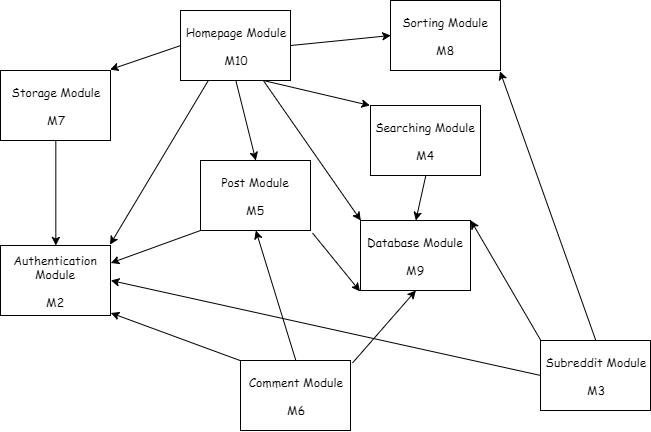
\includegraphics[width=17cm, height=11cm]{uses}
\caption{Use hierarchy among modules}
\label{FigUH}
\end{figure}

\end{document}
